\chapter{A Tentativa de Aula com a Profª. Cassandra}\label{chp:LABEL_CHP_REL}

\section{Introdução}\label{sec:LABEL_CHP_REL_SEC_INTRO}

No dia 31 de outubro de 2018 Bruno esteve em reunião com a professora Cassandra, na qual foi realizada a entrevista que foi relatada na seção \ref{chp:LABEL_CHP_ENT_SEC_CASS}. Nesta reunião, foi acordado que no dia 14 de novembro o laboratório seria utilizado pela Cassandra em parceria conosco para ministrar uma aula no software \textit{JFractionLab}. Ficou acordado que chegaríamos no CAp às 13h para realizar a instalação do software nas máquinas do laboratório, para que às 13h50min (início do segundo tempo de aula) a Cassandra pudesse levar os alunos ao laboratório e ministrar a aula com o nosso auxílio.

O presente relato visa expor as experiências que vivemos naquele dia e as informações que recolhemos, bem como os problemas que enfrentamos e percebemos. Separamos os problemas em tópicos, e, para cada um deles, formulamos alguns questionamentos, que foram levados à DALPE. Na seção \ref{sec:LABEL_CHP_REL_SEC_PROBS}, ao final deste capítulo, estão discriminados estes tópicos, bem como os questionamentos formulados e as respostas que foram dadas a eles.

\section{Relato do Dia da Aula}\label{sec:LABEL_CHP_REL_SEC_REL}

\subsection{A Espera}\label{sec:LABEL_CHP_REL_SEC_REL_SUBSEC_ESP}

No dia 14 de novembro, quarta-feira, às 13 horas, chegamos no CAp para realizar a instalação do software nas máquinas, entretanto, a bolsista que estava responsável pelo laboratório naquele horário, que deveria chegar também às 13h, não estava presente. Fomos à DALPE e lá nos informaram que a única saída seria aguardar, pois não era possível entregar a chave do laboratório a uma pessoa que não possuísse vínculo com o CAp. Aguardamos, então que a bolsista chegasse, o que só se concretizou às 13h45min, cinco minutos antes do segundo tempo, horário combinado com a Cassandra para trazer os alunos ao laboratório.

Ao longo do tempo de espera, estivemos sentados em frente à porta do laboratório, e pudemos constatar que diversos alunos procuraram o LIE para utilizá-lo, mas o encontraram vazio, com a porta trancada.

\subsection{Problemas Estruturais Encontrados}\label{sec:LABEL_CHP_REL_SEC_REL_SUBSEC_PROB}

Na ocasião da chegada da bolsista, o laboratório foi aberto por ela e constatou-se que estava trancada a porta interna do laboratório, que dá acesso à área onde fica o computador utilizado pelos bolsistas e outros materiais relevantes. A bolsista responsável naquele momento disse que apenas um outro bolsista tinha a chave, mas que ele já havia ido embora. Relatou que a DALPE não possuía cópia da chave, e que seria necessário chamar um funcionário da manutenção.

Em seguida, a bolsista foi até o aparelho de ar condicionado e nós percebemos que, logo abaixo do aparelho, havia uma tomada externa, onde este se encontrava ligado, e, apoiado na caixa da tomada, havia um copo de guaraná natural aberto, completamente cheio de água. O ar condicionado, que havia sido deixado ligado enquanto o laboratório permaneceu trancado, estava com um vazamento de água, e o copo fora posicionado de modo a coletar a água que pingava; entretanto, por conta do tempo que o laboratório permaneceu trancado com o aparelho ligado sem ninguém para supervisioná-lo, o copo havia transbordado.

\begin{figure}[ht]
  \centering
  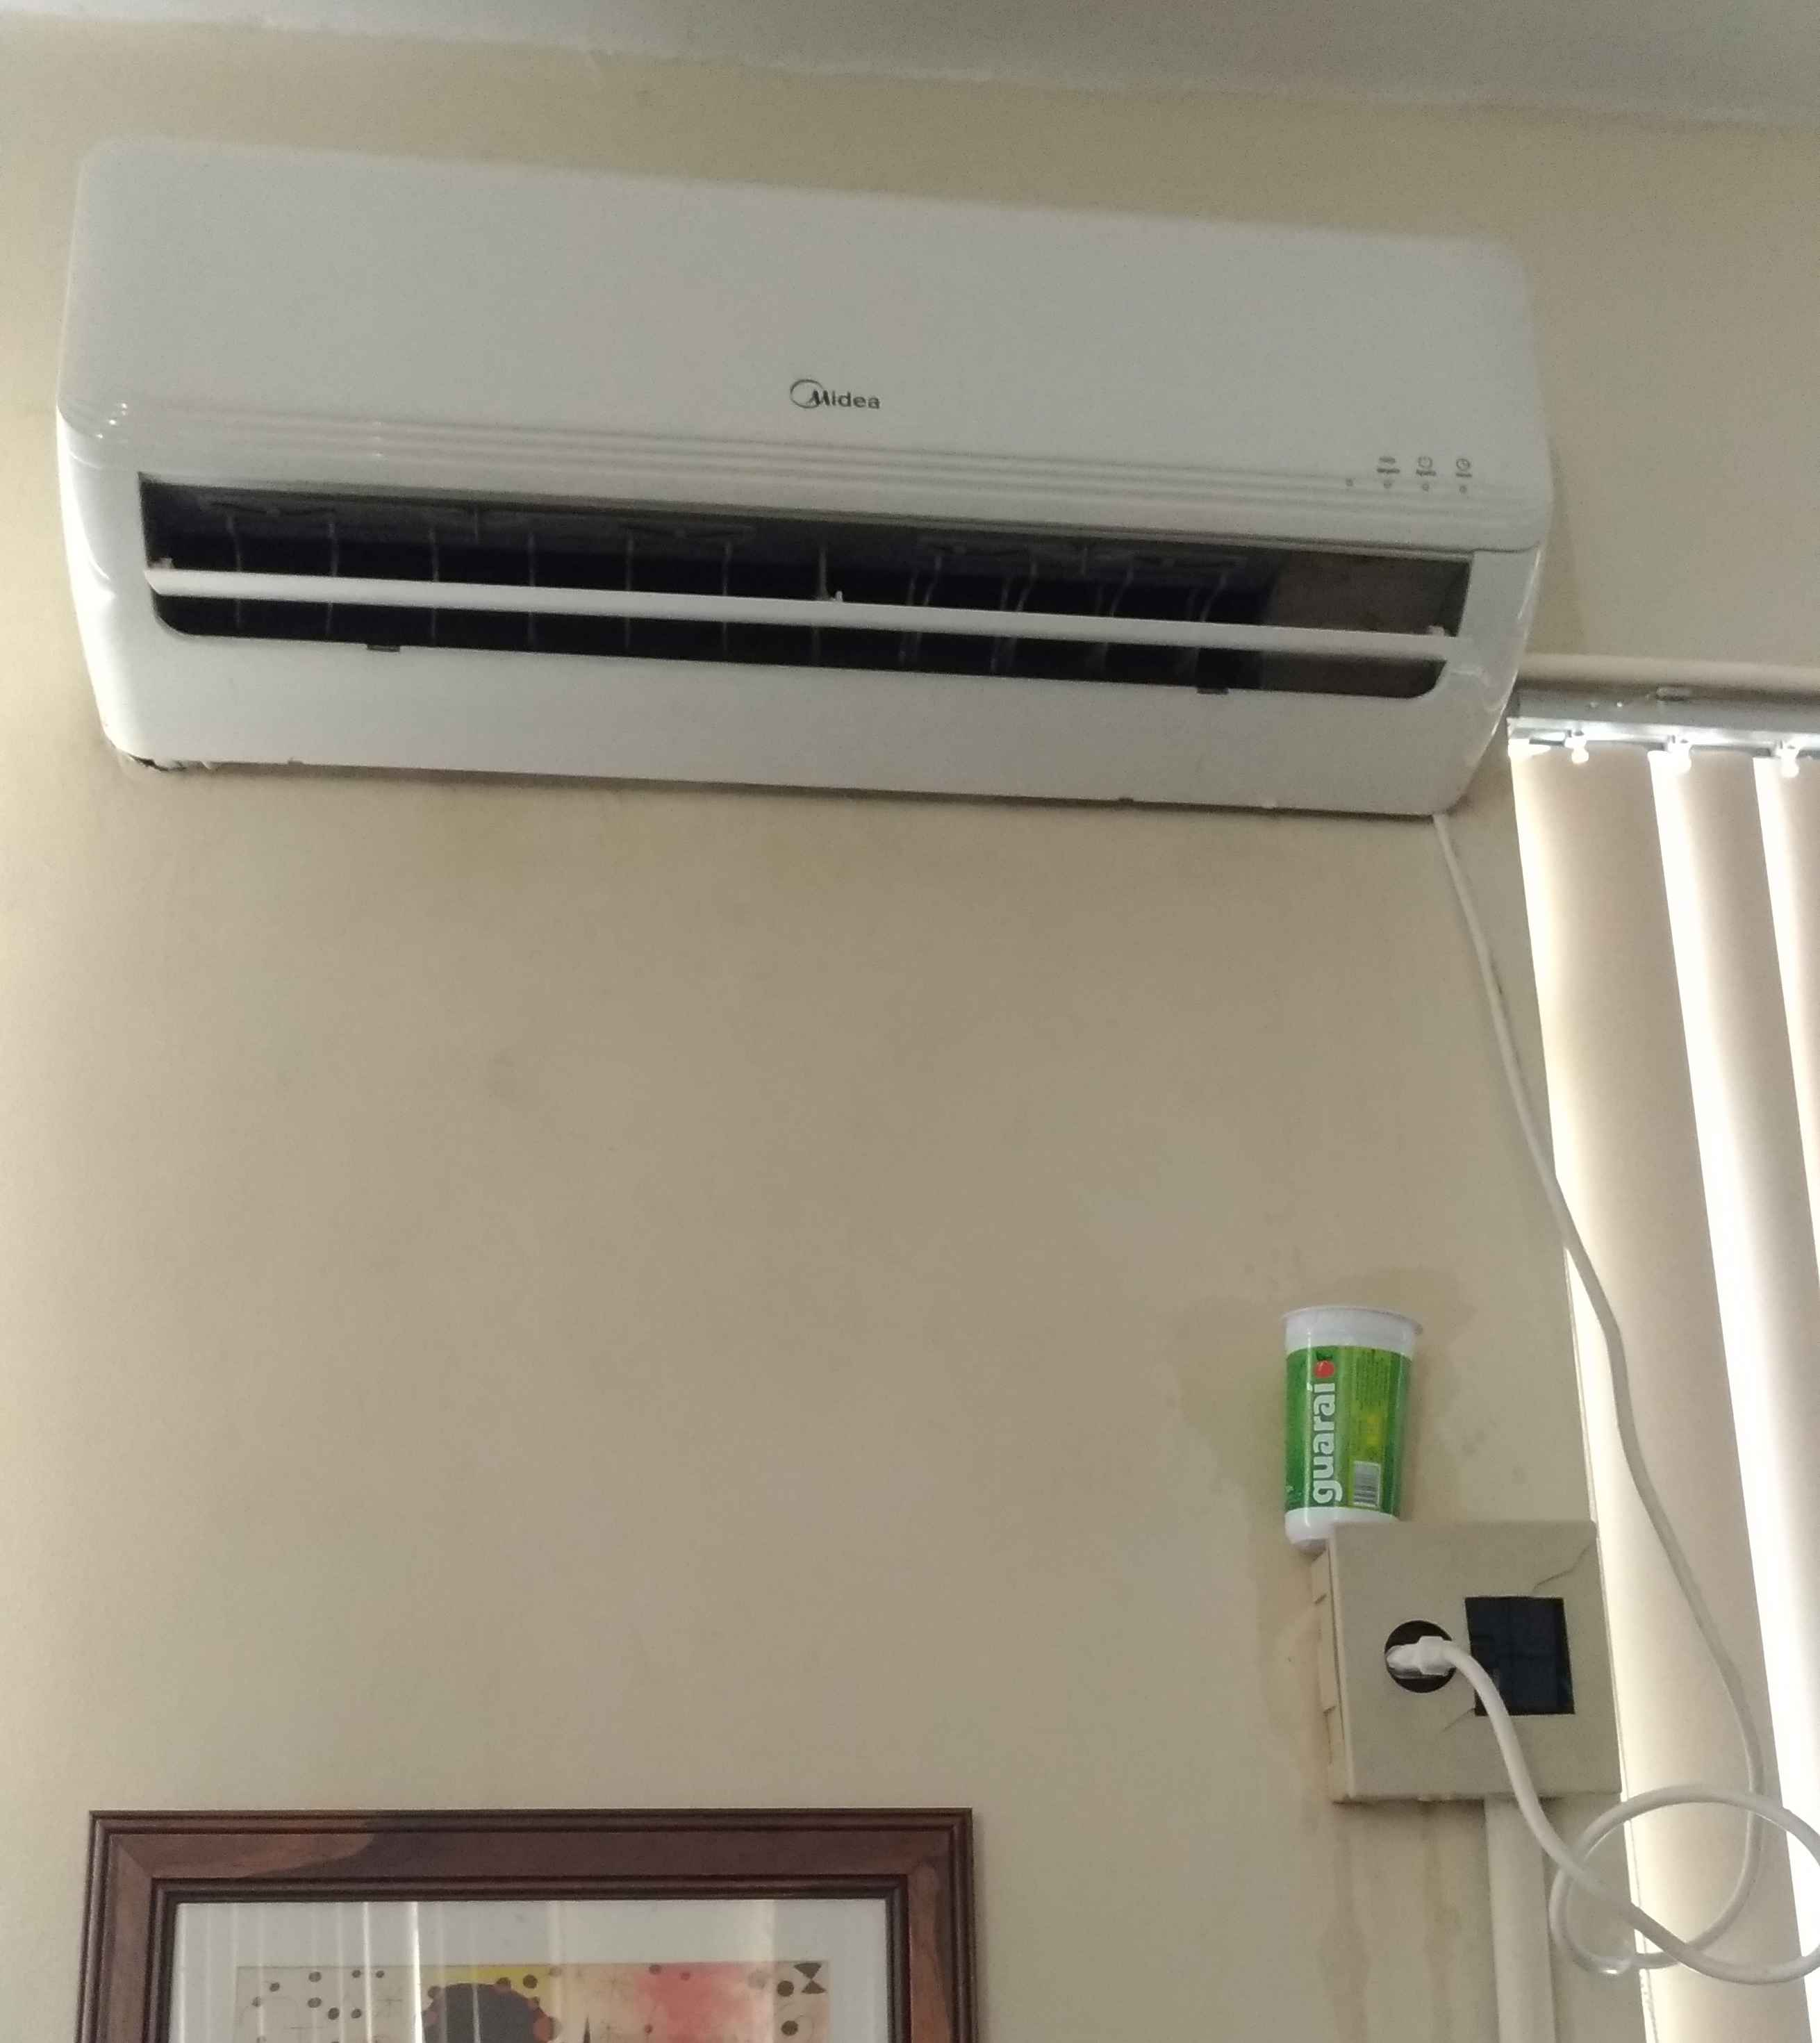
\includegraphics[width=0.7\textwidth]{imagens/copo.jpg}
  \caption{Ar condicionado pingando e copo sobre a tomada para coletar a água.}
  \label{fig:LABEL_FIG_COPO}
\end{figure}

A água que pingava e transbordava, então, havia molhado a caixa da tomada na qual o aparelho encontrava-se ligado naquele momento, bem como havia molhado o gabinete de um computador e uma das mesas dos computadores. Escorrendo pela parede para o chão, a água havia formado uma grande poça abaixo da mesa que fora molhada. A bolsista se mostrou chateada com a situação, reclamando, sozinha, quem alguém havia deixado o ar condicionado ligado ao sair do laboratório.

\begin{figure}[ht]
  \centering
  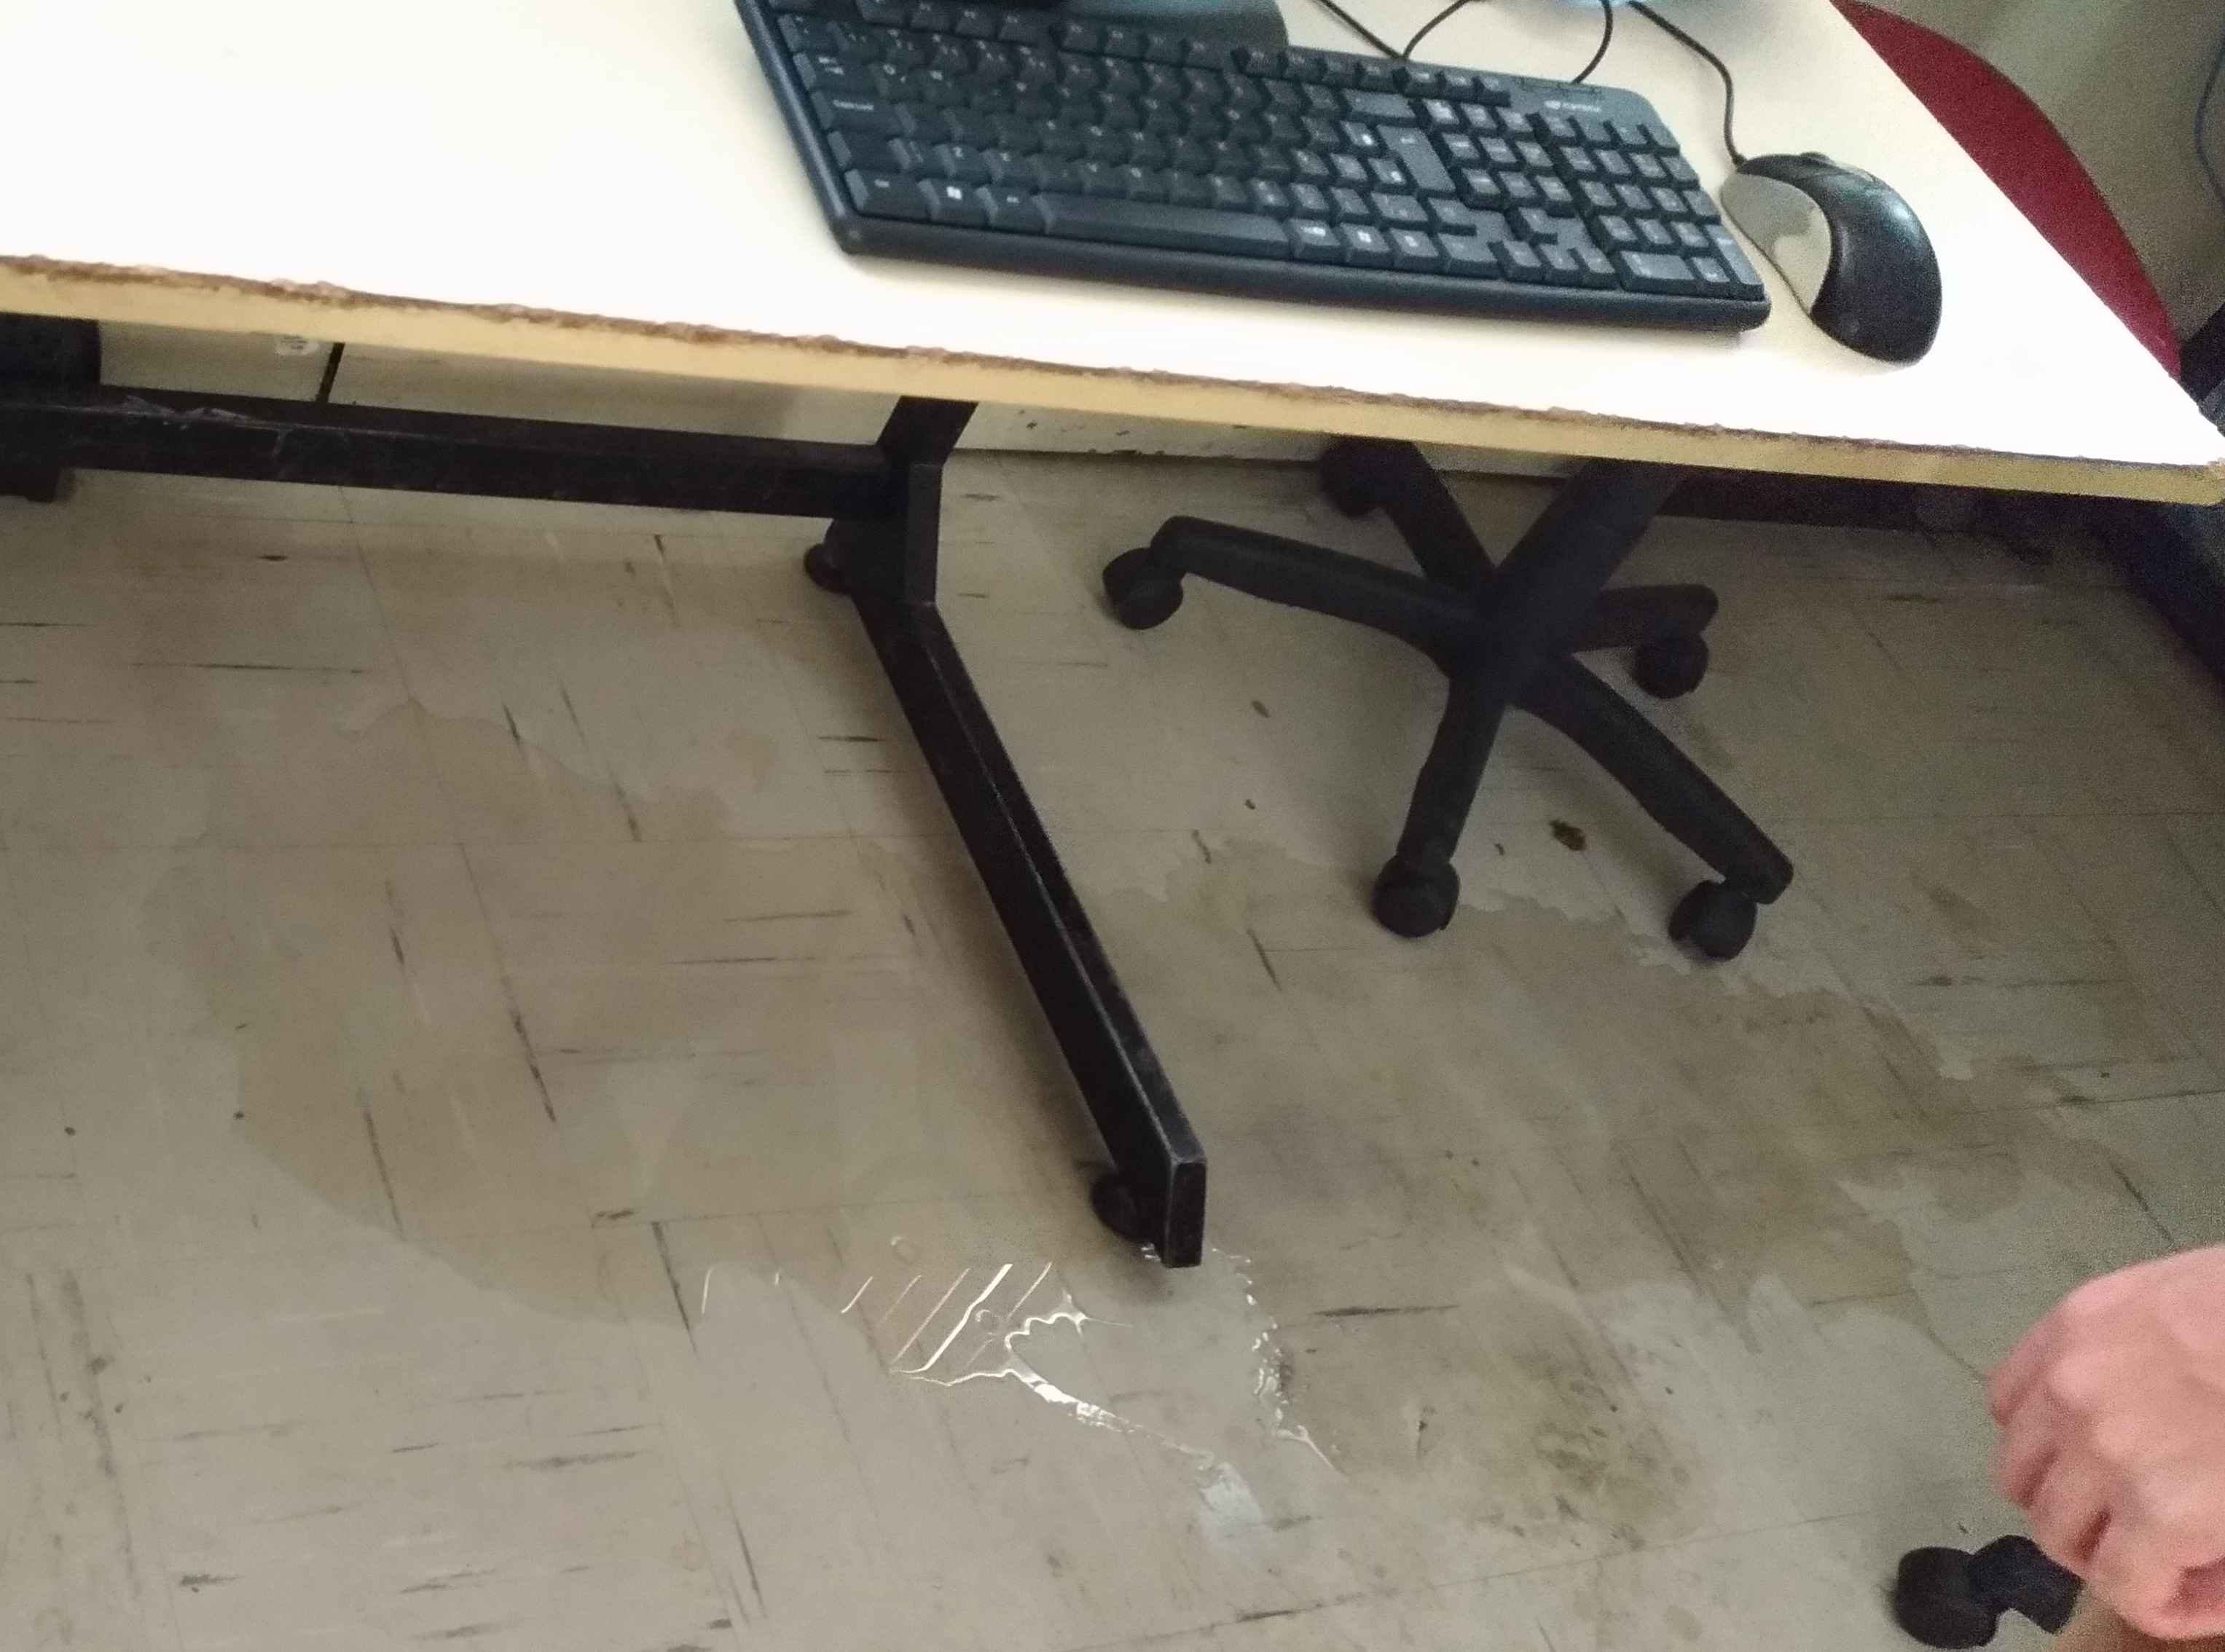
\includegraphics[width=0.9\textwidth]{imagens/poca.jpg}
  \caption{Poça formada no chão por conta do transbordamento do copo.}
  \label{fig:LABEL_FIG_POCA}
\end{figure}

Também foi observado que o laboratório possuía algumas cadeiras avariadas, com encosto e/ou assento rasgados, bem como uma cadeira cujo encosto havia sido removido, deixando os ferros que davam suporte ao encosto expostos, aumentando assim o risco de acidentes, principalmente com as crianças que frequentam o laboratório. 

Foi observado ainda que havia grande número de caixas de papelão, de conteúdo desconhecido, empilhadas atrás da porta do laboratório; e que a impressora do laboratório estava quebrada, com um papel anexado a ela, escrito “Em manutenção. Favor não ligar”.

Outra observação relevante é que o local onde o laboratório se encontra possui uma pilastra no meio da sala, o que dificulta o ministério de aulas. Além disso, foi possível observar colados nas paredes os avisos de relacionamento com o espaço que foram mencionados pela Profª. Isabel, da DALPE, na sua entrevista.

\begin{figure}[ht]
  \centering
  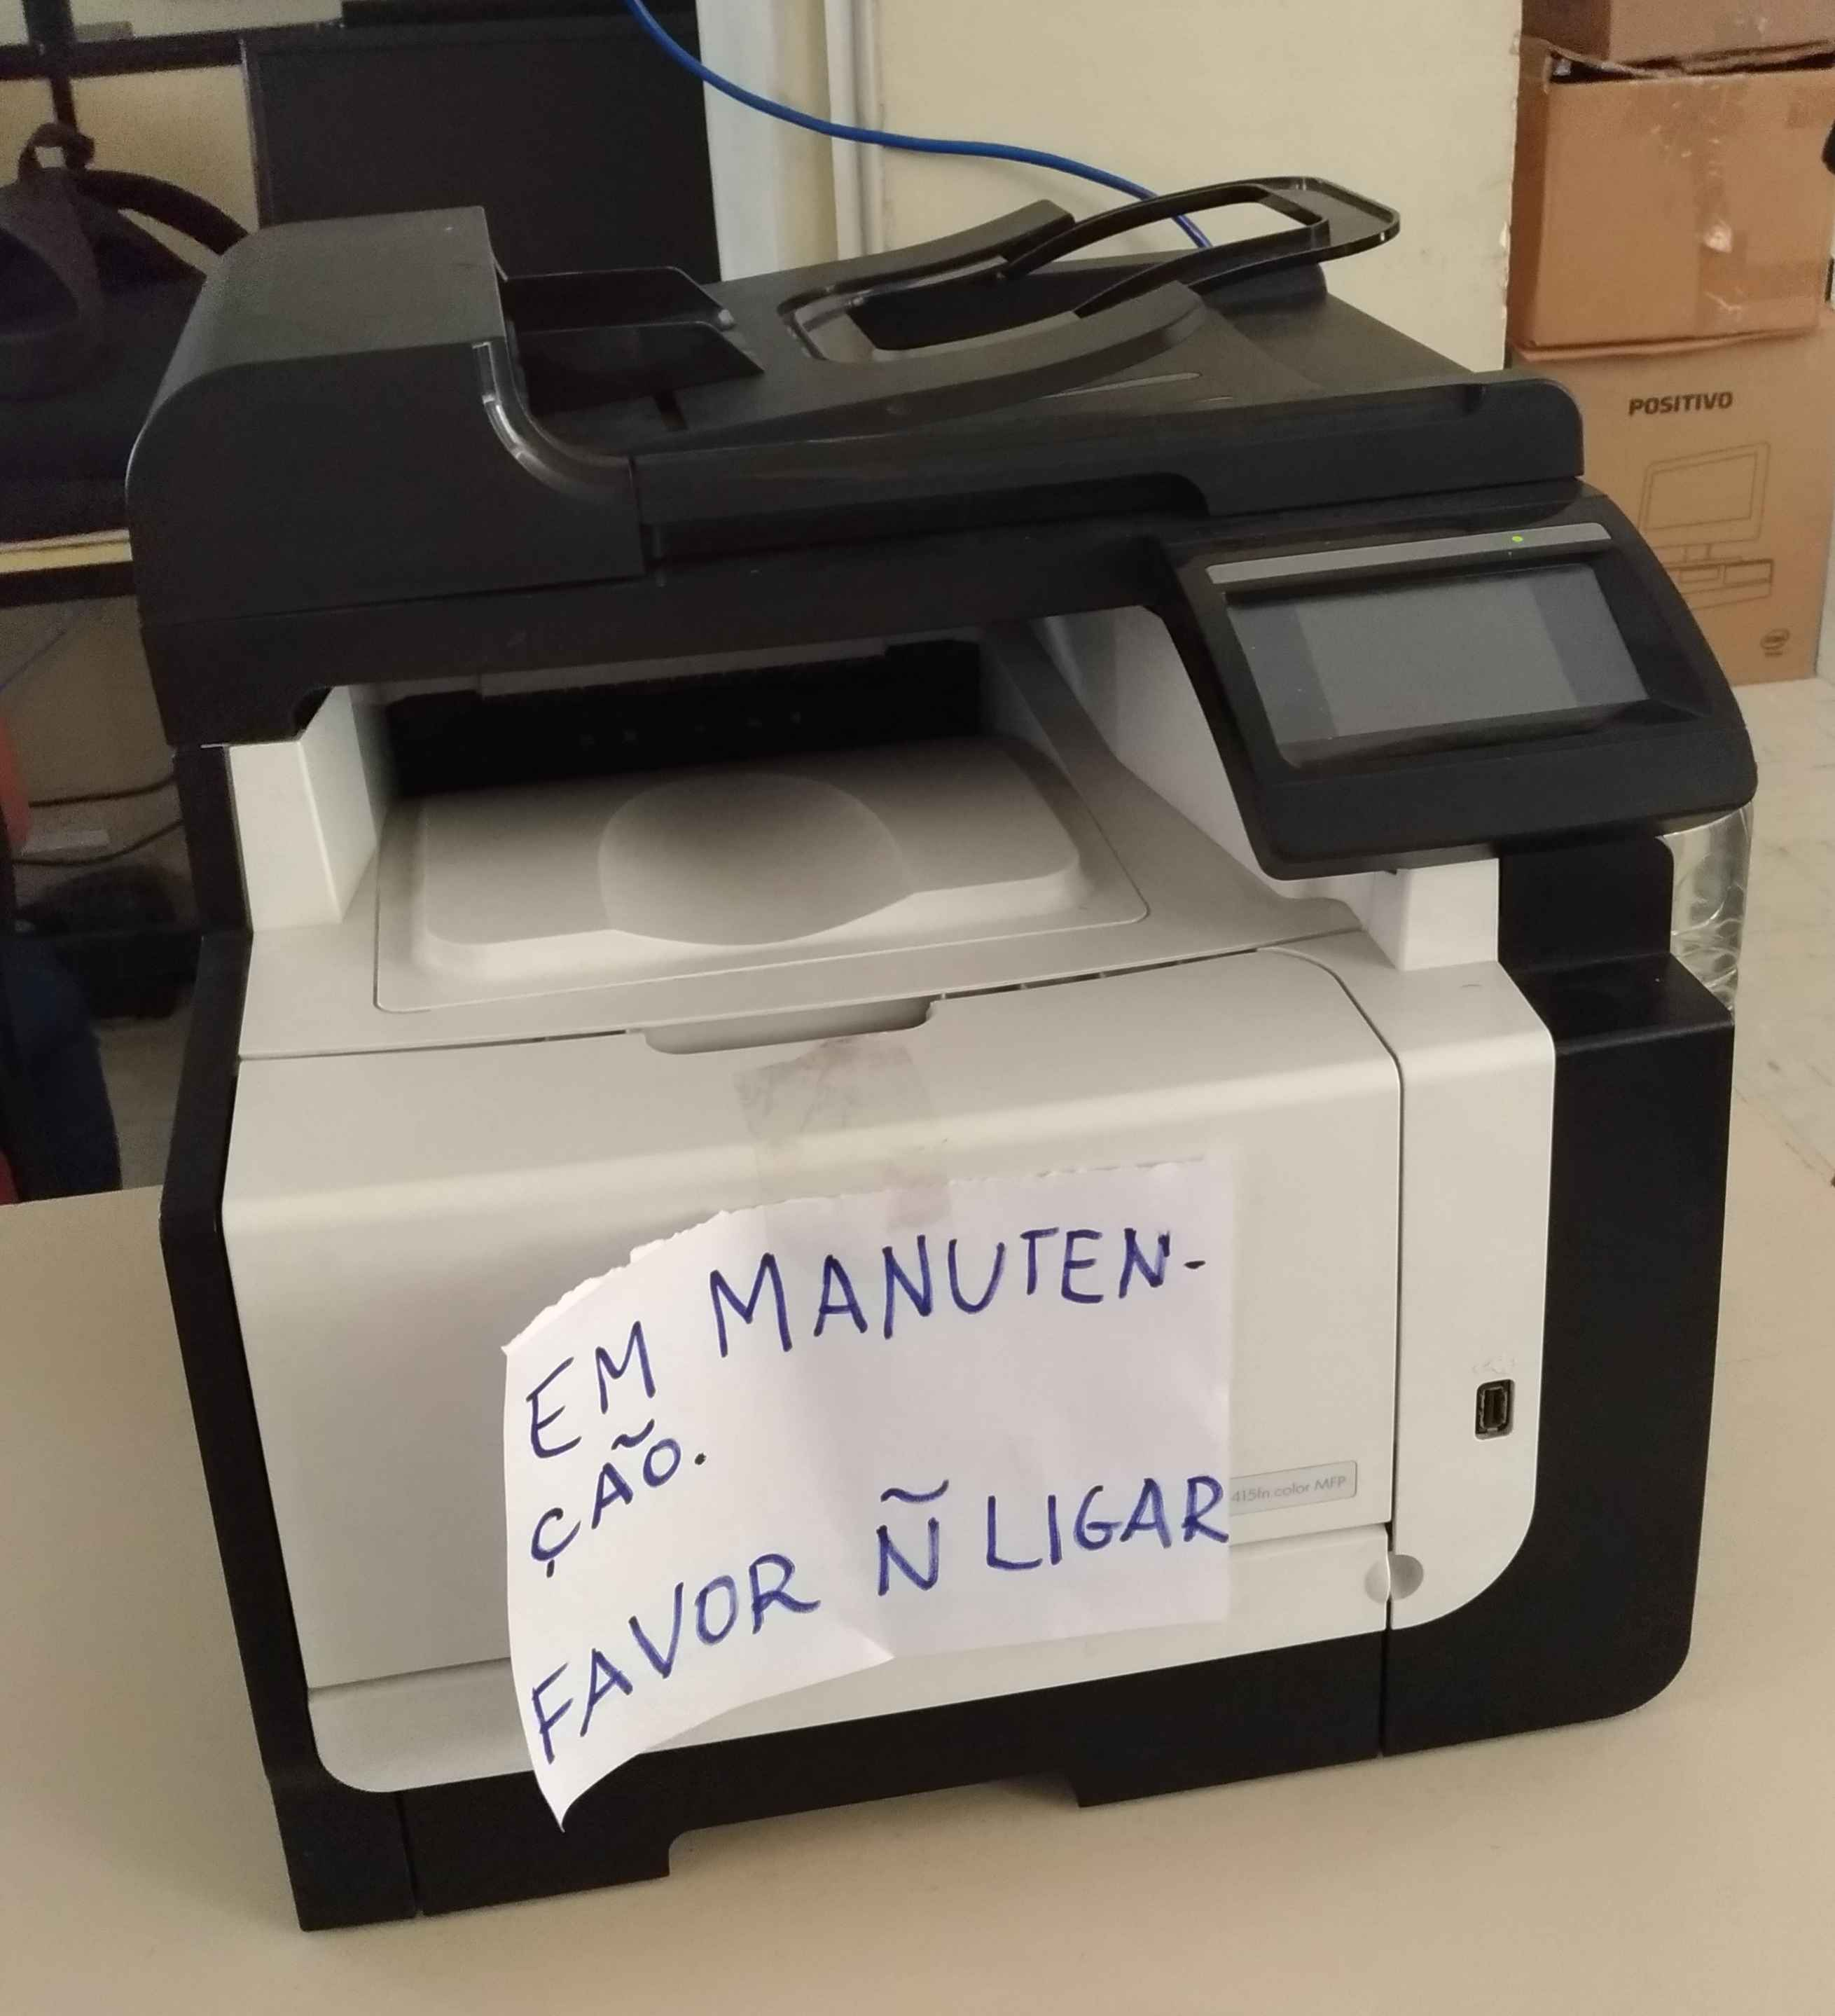
\includegraphics[width=0.8\textwidth]{imagens/impressora.jpg}
  \caption{Impressora com aviso de manutenção.}
  \label{fig:LABEL_FIG_IMP}
\end{figure}

\begin{figure}[ht]
  \centering
  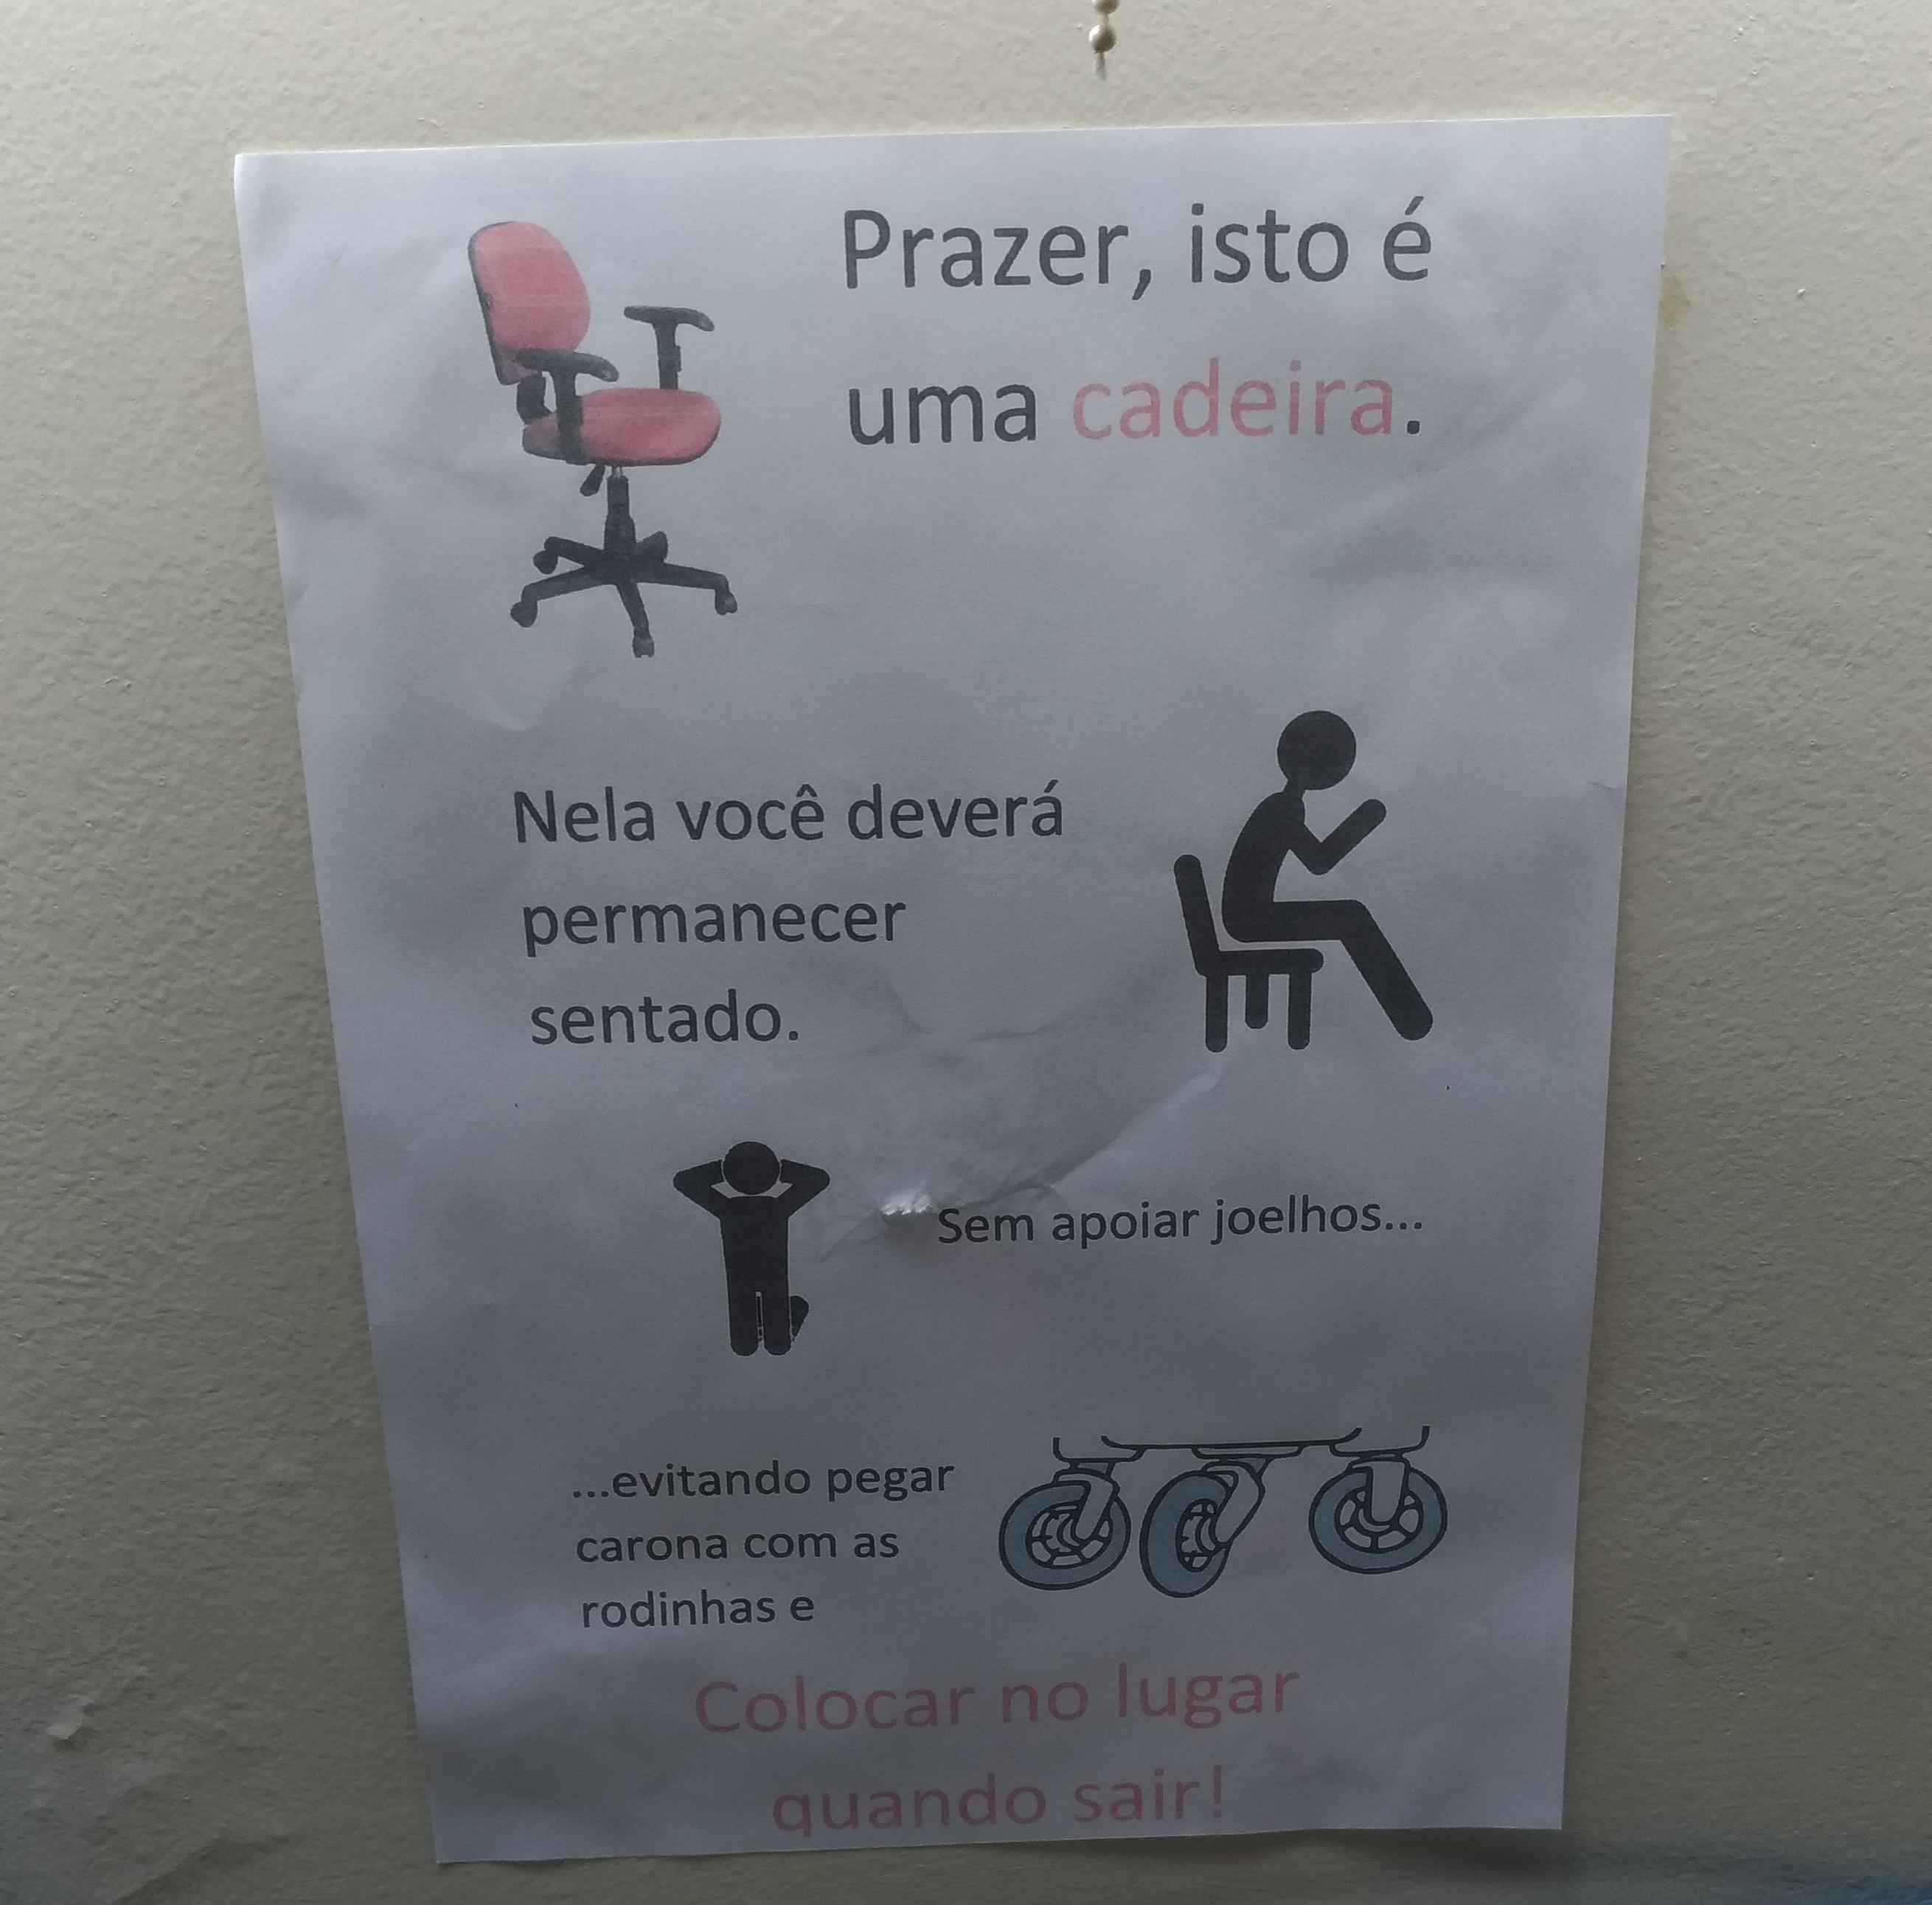
\includegraphics[width=0.8\textwidth]{imagens/aviso.jpg}
  \caption{Um dos avisos de relacionamento com o espaço.}
  \label{fig:LABEL_FIG_AVISO}
\end{figure}

\subsection{A Chegada dos Alunos}\label{sec:LABEL_CHP_REL_SEC_REL_SUBSEC_CHEG_AL}

Neste momento, a professora Cassandra chegou com os alunos do 5º (quinto) ano para a aula. Ao acomodá-los no laboratório, foi necessário pedir para que as crianças tomassem cuidado com a área que estava molhada, e instruí-las no sentido de que não seria possível utilizar os computadores daquela área. Após acomodar todos os alunos no laboratório, ela pediu para que nós falássemos com eles. Bruno então informou-os de que não seria possível utilizar o laboratório naquele momento pois ainda estava faltando instalar o programa que seria utilizado por eles, o que gerou grande frustração nos alunos, que apresentavam visível empolgação com a perspectiva de assistir uma aula no laboratório.

Ao recolher os alunos para levá-los de volta à sala de aula, Cassandra informou que poderia voltar ao laboratório no 4º (quarto) tempo de aula, às 16h30min, caso o problema da instalação do software fosse solucionado em tempo hábil, ao que nos comprometemos em envidar esforços neste sentido.

\subsection{A Chegada da Manutenção}\label{sec:LABEL_CHP_REL_SEC_REL_SUBSEC_CHEG_MAN}

Enquanto os alunos estavam no laboratório, o funcionário da manutenção que fora convocado para sanar o problema da porta interna trancada chegou, munido de uma escada de madeira e um cabo de vassoura. Devido à presença das crianças no laboratório, ele aguardou até que pudesse realizar seu trabalho. Após a retirada delas, posicionou a escada contra a porta e, subindo nela, comentou com a bolsista: “de novo essa porta, é?”.

Interpelada, a bolsista informou que não era a primeira vez que este problema acontecia; ao contrário, era um problema recorrente, e questionada acerca do porquê da DALPE não possuir uma cópia da chave, ela não soube explicar; questionado, o funcionário informou que o setor de manutenção não possui cópia daquela chave, mas também não deu explicações do porquê. A bolsista ainda informou que os seguranças do CAp, que guardam a chave do laboratório quando este não está em uso, também não possuem cópia da chave da porta interna.

Uma vez no topo da escada, o funcionário pegou o cabo de vassoura e passou-o por uma abertura acima da porta, de modo que este alcançasse a maçaneta pelo lado de dentro. Após alguns minutos de esforço, o funcionário conseguiu abrir a porta por dentro e deixou o recinto levando a escada e o cabo de vassoura, retornando logo em seguida com um pano de chão e um balde, para secar a poça d’água formada pelo ar condicionado que estava pingando.

Questionado se o problema era recorrente, ele disse que era bastante frequente que os bolsistas esquecessem de esvaziar o copo que coletava as gotas que pingavam e este transbordasse, formando assim a poça no chão e molhando os objetos ao redor do aparelho. A bolsista presente aproveitou a ocasião para esvaziar o copo. 

\subsection{A Tentativa de Instalação do Software}\label{sec:LABEL_CHP_REL_SEC_REL_SUBSEC_INST}

Logo em seguida, questionamos a bolsista acerca da instalação do \textit{JFractionLab}, ao que fomos informados de que não seria possível realizá-la pois ela não possuía a senha de administrador das máquinas. A bolsista orientou-nos no sentido de que a instalação de novos programas deveria ser realizada por meio de solicitação à DALPE, e que, caso a solicitação fosse aprovada, os bolsistas se encarregariam de realizar a instalação dos programas solicitados e de informar quando o laboratório estaria disponível para utilização com estes programas.

Interpelada a respeito de quem seria responsável por realizar a avaliação técnica da solicitação de instalação de software, uma vez que a DALPE não possui funcionário com tal competência, a bolsista informou que um outro bolsista, o que possui a senha de administrador, faria a avaliação e aprovação ou não da solicitação, bem como o procedimento de instalação no caso de aprovação.

Uma vez que ficou claro que a decisão estava na mão de um bolsista, Filipe, que possuía o telefone deste bolsista, perguntou se seria possível realizar a instalação do programa obtendo uma autorização por telefone, ao que a bolsista que estava no laboratório aquiesceu, com a restrição de que a instalação fosse realizada por nós, alunos de computação, pois ela era aluna de um curso não relacionado à informática e não julgava possuir as competências técnicas necessárias para o procedimento de instalação.

Efetuada a ligação para o bolsista responsável pelas instalações de software e explicada a situação, a autorização foi concedida e a senha de administrador foi passada para a bolsista do horário, que a colocou em uma das máquinas para que a instalação fosse realizada. Realizamos, então, este procedimento, entretanto, a instalação não foi concluída com êxito, pois o \textit{JFractionLab} precisa de um software adicional para funcionar: o \textit{Java}.

Ao ser informada da situação, a bolsista disse que o \textit{Java} poderia ser instalado somente mediante autorização do outro bolsista. Em nova ligação telefônica, explicada a situação, o bolsista recusou o pedido de instalação, alegando que as máquinas não possuíam capacidade de hardware suficiente para rodar o \textit{Java}. Filipe questionou tal decisão, uma vez que Bruno já havia obtido um relatório do hardware da máquina à qual tinham acesso de administrador, e este relatório demonstrava a plena capacidade de hardware daquela máquina para atender os requisitos necessários à instalação do \textit{Java}; entretanto, o bolsista foi irredutível, solicitou que o telefone fosse passado para a bolsista do horário e a orientou no sentido de não permitir a instalação do \textit{Java}. Questionado acerca da presença, na máquina, de outros softwares instalados que possuíam requisitos técnicos superiores ao \textit{Java}, o bolsista não deu quaisquer explicações e se manteve irredutível.

\subsection{A Procura por Alternativas}\label{sec:LABEL_CHP_REL_SEC_REL_SUBSEC_PROC_ALT}

Começamos então a avaliar alternativas que pudessem executar o \textit{JFractionLab} sem a presença do \textit{Java}. Inicialmente, pensamos em procurar o software em algum site de jogos, de modo que ele rodasse em um navegador, e, se não encontrássemos, tentar hospedá-lo em algum servidor que possuísse o \textit{Java}; entretanto, esta alternativa rapidamente se revelou inviável, pois os softwares em \textit{Java} que rodam em navegadores dependem de um \textit{plug-in}, que por sua vez depende da instalação do \textit{Java}.

Foi avaliada então a alternativa de realizar uma portabilidade automática de código fonte para uma outra linguagem, uma vez que o \textit{JFractionLab} é software livre e possui código aberto. Uma vez que o software estivesse em outra linguagem, seria possível executá-lo sem a presença do \textit{Java}.

Entretanto, os serviços de portabilidade automática encontrados se limitavam a programas pequenos, a menos que fosse realizada a compra de pacotes \textit{premium}, e o \textit{JFractionLab} possui código fonte muito extenso, inviável de ser portado utilizando os planos gratuitos oferecidos por esses serviços.

Além disso, uma pesquisa revelou que os programas portados utilizando esses serviços em geral resultavam em programas com muitos erros, que precisavam ser consertados manualmente, o que levaria muito tempo e não daria qualquer garantia de que o software portado funcionaria da mesma forma que o original, tornando, então, esta alternativa inviável.

Diante da falta de alternativas, informamos à professora Cassandra que não seria possível utilizar o laboratório naquele dia. Realizamos, então, a entrevista com a bolsista presente no laboratório e retiramo-nos da escola mais ou menos às 17 horas.

\section{Dificuldades que Enfrentamos}\label{sec:LABEL_CHP_REL_SEC_PROBS}

\subsection{O Atraso da bolsista}\label{sec:LABEL_CHP_REL_SEC_PROBS_SUBSEC_ATR}

A bolsista que deveria chegar às 13 horas chegou apenas às 13:45. Neste interstício, o laboratório permaneceu trancado, impossibilitando tanto a realização do trabalho a que nos propomos quanto o uso por parte dos alunos que procuraram o laboratório e o encontraram fechado.

\subsubsection{Questionamentos levados ao CAp}

Vários bolsistas se atrasam, ou foi apenas esta bolsista? Esta bolsista se atrasa com frequência, ou foi um caso isolado? Os bolsistas atrasados sabem do impacto que podem causar ao laboratório ao se atrasarem?

\subsubsection{Resposta do CAp}

Os bolsistas eventualmente se atrasam por conta do deslocamento do Fundão (campus principal da UFRJ) para o colégio. Esse é o caso da Ingrid. Se tivesse sido realizado um contato anterior com ela, salientando a importância da pontualidade neste dia, a situação poderia ter sido contornada.

Cabe ressaltar que a posição do bolsista é de mero auxiliar das atividades do laboratório, e qualquer professor pode utilizá-lo sem a presença do bolsista, basta que solicite a chave. Dessa forma, o atraso de um bolsista não se configura, a princípio, como impeditivo para a realização de uma atividade no laboratório. Por conta disso, caso a presença dele seja imprescindível para a realização de uma atividade, isso deve ser avisado com antecedência. O simples fato de haver uma atividade marcada na planilha de aulas do laboratório não configura necessidade da presença do bolsista no laboratório.

\subsection{A Porta interna trancada}\label{sec:LABEL_CHP_REL_SEC_PROBS_SUBSEC_POR}

Na ocasião da chegada da bolsista foi constatado que a porta interna do laboratório, que dá acesso à área onde fica o computador utilizado pelos bolsistas e outros materiais relevantes, estava trancada, e o único bolsista que possuía a chave daquela porta já havia deixado o Colégio.

\subsubsection{Questionamentos levados ao CAp}

Quem instalou a porta só forneceu uma cópia da chave? Por que essa cópia ficou com o bolsista, ou para quem foram dadas as outras? Quem é responsável por tirar cópias da chave? Por que essas cópias ainda não foram tiradas?

\subsubsection{Resposta do CAp}

A porta interna não possui fechadura, apenas maçaneta. Não sabemos o que ocorreu neste dia, mas pode ser que a porta estivesse apenas emperrada. A Ingrid é uma bolsista que está conosco há pouco tempo, talvez ela tenha se confundido e achado que a porta estava trancada.

\subsection{O Ar condicionado pingando}\label{sec:LABEL_CHP_REL_SEC_PROBS_SUBSEC_AC}

Um dos aparelhos de ar condicionado do laboratório está com um vazamento de água para a parte interna do laboratório. É um problema grave, pois está molhando tanto uma tomada, o que pode levar a um curto circuito e em último caso a um incêndio; quanto um computador, que é um equipamento caro.

\subsubsection{Questionamentos levados ao CAp}

De quem é a responsabilidade de chamar a manutenção? Por que este responsável não chamou? Caso a manutenção já tenha sido chamada, por que ela não veio?

\subsubsection{Resposta do CAp}

A manutenção do ar condicionado do laboratório faz parte da manutenção de todos os aparelhos de ar condicionado da escola. No início de 2018 havia apenas um aparelho com defeito. Agora, quando voltamos às aulas em 2019, já temos sete aparelhos com defeito. Já foi realizado chamado de manutenção e esta será feita no sábado anterior ao carnaval, daqui a poucos dias.

\subsection{As Cadeiras avariadas}\label{sec:LABEL_CHP_REL_SEC_PROBS_SUBSEC_CAD}

Há diversas cadeiras avariadas dentro do laboratório, que podem causar acidentes e oferecem risco aos alunos que o utilizam.

\subsubsection{Questionamentos levados ao CAp}

Por que cadeiras avariadas continuam dentro do laboratório? De quem é a responsabilidade de solicitar a troca das cadeiras? Este responsável solicitou a troca? Se sim, por que ela ainda não aconteceu?

\subsubsection{Resposta do CAp}

A substituição das cadeiras do laboratório será realizada quando houver cadeiras novas disponíveis. A compra de cadeiras novas já foi solicitada, e segue os mesmos trâmites das outras compras da UFRJ.

\subsection{As Caixas atrás da porta}\label{sec:LABEL_CHP_REL_SEC_PROBS_SUBSEC_CAIX}

Na ocasião da nossa visita, havia diversas caixas armazenadas atrás da porta do laboratório, prejudicando a circulação de pessoas, impedindo a abertura completa da porta e oferecendo risco em potencial às crianças.

\subsubsection{Questionamentos levados ao CAp}

O conteúdo das caixas pertencia ao laboratório? Existe algum local no CAp destinado para armazenamento de caixas desse tipo?

\subsubsection{Resposta do CAp}

A sala na qual o laboratório se encontra hoje é uma sala adaptada, e nós temos muito pouco espaço no colégio como um todo - há setores que não possuem sala para funcionar. Temos consciência de que a sala é inadequada para um laboratório, mas não há o que fazer. Não podemos construir mais salas pois o prédio onde funciona o colégio pertence à Prefeitura do Rio de Janeiro, e não à UFRJ.

\subsection{A Impressora quebrada}\label{sec:LABEL_CHP_REL_SEC_PROBS_SUBSEC_IMP}

Na ocasião da nossa visita, a impressora estava quebrada e sobre ela estava colada uma folha, na qual estava escrito: “Em manutenção. Favor não ligar”. Este problema impede o atendimento à forte demanda de impressões que chega ao laboratório, tanto da parte dos alunos, que precisam imprimir trabalhos; quanto da parte dos professores, que precisam imprimir provas.

\subsubsection{Questionamentos levados ao CAp}

Quem é responsável por solicitar suporte e manutenção para a impressora? Quem realiza este suporte? A manutenção já foi solicitada? Se sim, por que a manutenção ainda não foi atendida pelo suporte?

\subsubsection{Resposta do CAp}

A manutenção da impressora já foi solicitada, entretanto a TIC/UFRJ possui poucos funcionários e muitos chamados, e até agora não conseguimos que o atendimento fosse realizado. Solicitamos também ao CFCH, mas ele possui apenas um funcionário para manutenção na área de informática, e ele é responsável por todos os laboratórios e computadores administrativos do CFCH. Infelizmente a manutenção realmente demora a vir.

\subsection{A Pilastra no meio da sala}\label{sec:LABEL_CHP_REL_SEC_PROBS_SUBSEC_PIL}

Observamos nas entrevistas que os professores tem dificuldade de ministrar suas aulas no laboratório por conta da pilastra presente no meio da sala, que não permite que o professor tenha visão completa da turma enquanto ministra a aula. Foi levantada também a hipótese de que a pilastra na sala atua como fator desencorajador para que os professores utilizem o laboratório.

\subsubsection{Questionamentos levados ao CAp}

Houve algum processo de decisão sobre o local do laboratório? Se sim, por que foi escolhida uma sala inadequada?

\subsubsection{Resposta do CAp}

A sala na qual o laboratório se encontra hoje é uma sala adaptada, e nós temos muito pouco espaço no colégio como um todo - há setores que não possuem sala para funcionar. Temos consciência de que a sala é inadequada para um laboratório, mas não há o que fazer. Não podemos construir mais salas pois o prédio onde funciona o colégio pertence à Prefeitura do Rio de Janeiro, e não à UFRJ.

\subsection{Somente um bolsista possui a senha de administrador}\label{sec:LABEL_CHP_REL_SEC_PROBS_SUBSEC_PSWD}

Na ocasião da nossa visita, foi-nos relatado pela bolsista do horário que a única pessoa que possui as senhas de administrador dos computadores é um bolsista. Além do risco de ter apenas uma pessoa de posse das senhas de administrador, o fato desta pessoa ser um bolsista deixa a administração técnica do laboratório a cargo de alguém que não possui vínculo com o colégio.

\subsubsection{Questionamentos levados ao CAp}

Porquê apenas um bolsista possui a senha de administrador? A Direção Geral, DALPE ou outras coordenações sabem da senha de administrador? Existe alguma política para acesso a esta senha?

\subsubsection{Resposta do CAp}

Os bolsistas se organizam entre si com a senha de administrador, pois, por conta de não termos pessoal especializado para a manutenção do laboratório, esta acaba se tornando um encargo deles. Não exercemos maior controle sobre isso por falta de capacidade técnica.

\subsection{A Requisição de instalação de software é avaliada por um bolsista}\label{sec:LABEL_CHP_REL_SEC_PROBS_SUBSEC_REQ_INST}

Na ocasião da nossa visita, era necessário instalar um software nos computadores do laboratório, ao que nos foi informado que deveria ser realizada uma requisição de instalação de software, e que esta seria avaliada pelo bolsista que possui a senha de administrador. Por se tratar de uma decisão técnica relevante sobre o laboratório como um todo, esta deveria ser tomada por um profissional de formação comprovada, que possuísse vínculo com o CAp e fosse responsável pelo laboratório.

\subsubsection{Questionamentos levados ao CAp}

Existe algum processo de avaliação formal de requisição de instalação de software, ou este fica apenas a cargo do bolsista?

\subsubsection{Resposta do CAp}

Não possuímos pessoal com a formação técnica necessária para avaliar as requisições de instalação de software, por isso elas ficam a cargo dos bolsistas. Não é o cenário ideal, mas foi dessa forma que conseguimos nos organizar.

\subsection{A Bolsista não possuía capacitação para instalar softwares nos computadores}\label{sec:LABEL_CHP_REL_SEC_PROBS_SUBSEC_INST_SOFT}

A bolsista que estava no laboratório quando estivemos nele nos relatou que não sabia instalar novos softwares nos computadores, o que é uma tarefa relativamente simples.

\subsubsection{Questionamentos levados ao CAp}

Os bolsistas do laboratório necessitam de um conhecimento mínimo de informática para atuarem no CAp? Existe alguma capacitação básica dos bolsistas?

\subsubsection{Resposta do CAp}

A capacitação dos bolsistas é incentivada frequentemente, pois encaramos isso como uma maneira de complementar a formação deles, entretanto, nem todos os bolsistas tem conhecimentos técnicos, bem como nem todos os bolsistas tem conhecimentos pedagógicos. É por isso que, na seleção dos bolsistas, procuramos formar uma equipe multidisciplinar que atenda a todas as necessidades. A bolsista que esteve com vocês tem formação na área pedagógica, e não na técnica.

\section{O Que Aprendemos}\label{sec:LABEL_CHP_REL_SEC_CONC}

Quanto aos problemas mais estruturais, cuja solução não depende diretamente da atuação do CAp, como a manutenção do ar condicionado, onde a única saída é esperar que a manutenção venha, não vislumbramos solução mais imediata que esteja ao alcance de ser desenvolvida pelo CAp.

Entretanto, refletindo sobre os problemas expostos, chegamos à conclusão de que os que são de ordem técnica e pedagógica seriam sanados, ou pelo menos amenizados, com a presença do “docente do LIE”, um professor com formação tanto pedagógica quanto computacional, alocado para se responsabilizar pelo LIE e para transformar o laboratório em um verdadeiro recurso pedagógico no colégio.

Nesse contexto, o docente do LIE é responsável tanto pela manutenção do espaço e dos recursos tecnológicos quanto pela elaboração de projetos pedagógicos do laboratório, em consonância com o projeto pedagógico do colégio. O docente do LIE é responsável, ainda, por oferecer suporte tanto técnico quanto pedagógico aos professores que utilizarem o laboratório. Atualmente, no CAp, esse suporte, quando existe, é ineficaz; e o projeto pedagógico do laboratório é inexistente. Em poucas palavras, o docente do LIE é responsável por fazer a conexão entre as disciplinas do currículo regular e os recursos tecnológicos presentes no colégio.
